\section {Cenni teorici}

\begin {frame}
\frametitle {Modellazione formale}
\begin{columns}
	\column{.3\textwidth}
	\begin{block}
		{Modello} rappresentazione fedele, ma astratta, di un sistema che permette di ricavare informazioni tramite processi logici, anzich\'e sperimentali
	\end{block}
	\begin{block}
		{Modello formale} modello matematico che non soffre di \alert{inconsistenze}, \alert{ambiguit\`a} e \alert{incompletezze} e su cui \`e possibile effettuare un'analisi \alert{automatizzata}
	\end{block}
	\column{.6\textwidth}
	\begin{itemize}
		\item Il formalismo scelto deve essere il pi\`u adatto possibile al sistema da modellare
		\item Non esiste un formalismo universale e spesso \`e necessario integrare le informazioni ottenute da pi\`u formalismi
		\item Un formalismo adatto alla comprensione umana \`e di difficile analisi per una macchina e viceversa
		\item Nel caso di \alert{sistemi reattivi} i formalismi concreti sono riconducibili a grafi e qualsiasi analisi sul modello astratto \`e riconducibile alla ricerca di percorsi sul grafo sottostante
	\end{itemize}

\end{columns}
\end{frame}



\begin {frame}
\frametitle {Modellazione formale}
\framesubtitle {Problema}
Dovendo rappresentare tutti i possibili comportamenti del sistema, all'aumentare del numero di interazioni, si verifica un'\alert{esplosione dello spazio degli stati}:


	\begin{columns}
		\column{.3\textwidth}
		\visible<1->{
		\begin{block}{2 specie, 1 reazione}
			\includegraphics[width=\textwidth]{michaelis/prism2.png}
		\end{block}
	}
		\column{.3\textwidth}
		\visible<1->{
		\begin{block}{4 specie, 3 reazioni}
			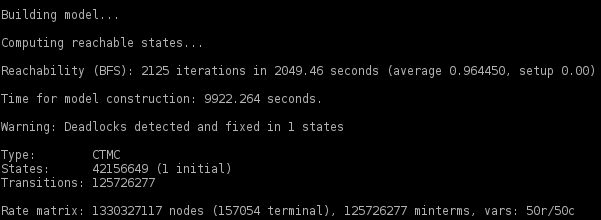
\includegraphics[width=\textwidth]{michaelis/prism.png}
		\end{block}
	}
		\column{.3\textwidth}
		\visible<1->{
		\begin{block}{5 specie, 3 reazioni}
			\includegraphics[width=\textwidth]{michaelis/prism3.png}
		\end{block}
		
			
		}
	\end{columns}
	


\end{frame}

\begin {frame}
\frametitle {Modellazione formale}
\framesubtitle {Soluzione: Astrazione}
\only<1>{\begin{columns}
	\column{.45\textwidth}
	\begin{equation*}
	E + S \xrightleftharpoons[k_{-1}]{k_1} ES \xrightarrow{k_2} E + P
	\end{equation*}
	\column{.1\textwidth}$\leadsto$
		\column{.45\textwidth}
		\begin{align*}
		r_1 &= k_1 [E][S]\\
		r_{-1} &= k_{-1}[ES]\\
		r_2 &= k_2 [ES]\\
		E &= r_1\downarrow E + r_{-1}\uparrow E + r_2 \uparrow E\\
		S &= r_1 \downarrow S + r_{-1} \uparrow S\\
		ES &= r_1 \uparrow ES + r_{-1} \downarrow ES + r_2 \downarrow ES\\
		P &= r_2 \uparrow P\\
		E &\underset{\{r_1, r_{-1}, r_2\}}\bowtie \left(S \underset{\{r_1, r_{-1}\}}\bowtie \left(ES \underset{\{r_2\}}\bowtie P\right)\right)
		\end{align*}
\end{columns}
}
\only<2>{\begin{columns}
		\column{.45\textwidth}
		\begin{equation*}
		S \xrightarrow{E} P
		\end{equation*}
		\column{.1\textwidth}$\leadsto$
		\column{.45\textwidth}
		\begin{align*}
		r &= \frac{V_{max} [S]}{K_M + [S]}\\
		{\color{gray}E }&{\color{gray}= r\oplus E}\\
		S &= r \downarrow S\\
		P &= r \uparrow P\\
		{\color{gray}E }&{\color{gray}\underset{\{r\}}\bowtie} S \underset{\{r\}}\bowtie P
		\end{align*}
	\end{columns}
}

\end{frame}

\iffalse

\begin {frame}[allowframebreaks]
\frametitle {Casi studio in letteratura}
\printbibliography
\end{frame}

\fi